
\documentclass[11pt]{article}

\usepackage{common}
\usepackage{amsmath}
\usepackage{graphicx}
\usepackage{float}
\usepackage{listings}
\usepackage[toc,page]{appendix}


\title{HW3: (Neural) Language Modeling}
\author{Nicolas Drizard \\ nicolasdrizard@g.harvard.edu \and Virgile Audi \\ vaudi@g.harvard.edu }
\begin{document}

\maketitle{}
\section{Introduction}

This assignment focuses on the task of language modeling, a crucial first-step for many natural language applications. In this report, we will present several count-based multinomial language models with different smoothing methods, an influential neural network based language model from the work of Bengio et al. (2003), and an extension to this language model which learns using noise contrastive estimation, as well as their implementation using Torch. We found this homework more challenging than the previous ones and encountered significant challenges that we will underline in this report. 


\section{Problem Description}

The goal of the language models presented in this report is to learn a distributed representation for words as well as probability distribution for word sequences. Language models are usually represented as the probability of generating a new word conditioned on the preceeding words:

$$ P(\boldsymbol{w}_{1:n}) = \prod\limits_{i=1}^{n-1}P(w_{i+1}|w_i)$$

\noindent To simplify the analysis, it is common to make the assumption that a word is influenced only by the $N$ words immediately preceeding it, which we call the context. Even with reasonably small values for $N$, building such models are extremely expensive computationally-wise as well as time-consuming if not ran on GPU. The joint proabibility of a sequence of 6 words taken from a vocabulary of 10 000 words could possibly imply training the model to fit up to $10^{4^6}-1 =10^{24}-1$ parameters.\\

\noindent The objective of this homework was to predict a probability distribution over 50 words at a given place in the sentence and based on the previous words.
To do so, we tried implementing N-grams models in an efficient manner. Due to computational limitations (no access to GPUs...), we faced difficulties training the Neural Network and focused our efforts on building strong count-based models to solve the problem of language modeling.


\section{Model and Algorithms}

We will now dive into more details of two types of models, i.e. count-based models and neural network models.

\subsection{Count-based Models}

The first models we implemented are based on the count of N-gram features. The main idea is here to implement n-gram multinomial estimates of $p(w_i|w_{i-n+1}, \hdots, w_{i-1})$. We will use different smoothing methods and compare their performance.

\paragraph{Maximum Likelihood Estimation}

The first approach is just to compute the maximum likelihood estimation $p_{ML}(w|c)$ with c the context (ie N-1 gram) and w the word predicted. This is done by simply counting the frequency of the N-gram: c-w in the training.

\[
	p_{ML}(w|c) = \frac{F_{c,w}}{F_c} = \frac{F_{c,w}}{\sum_i F_{c,w_i}}
\]

with $ F_{c,w} = \sum_i \mathbb{1}(w_{i-n+1:i-1}=c, w_i=w)$.


We applied this method up to 5-grams. But the results are not very impressive. First, the long tail in the words distribution is not properly represented as we consider the number of occurences of such words as the ground truth. Second, this method works for one context at a time but it should be more interesting to weight and combine them.

\paragraph{Laplace smoohting}

This approach handles the first issue where we want to have a better representation for the words in the tail. Here we simply add an off-set to each count $\hat{F}_{c,w} = F_{c,w} + \alpha $.

We can use the validation set to tune the $\alpha$ parameter while optimizing its perplexity. We applied this pipeline on the validation set from Kaggle.

\paragraph{Witten-Bell smoothing}

Here we tackle the second issue of the MLE. The idea is to combine lower order models together to use as much information as possible. The global idea is to use recursivity: 

\[
	p(w|c) = \lambda p_{ML}(w|c) + (1 - \lambda)p(w|c')
\]

with c' the lower order context (if c is the N-1 gram, c' is the N-2 gram). We stop it when c' is empty and then use the prior on the words distribution from the train (ie the frequency of the word w only). 

Witten and Bell suggested a way to compute the constant: $\lambda = \frac{N1_c}{F_c + N1_c}$ with $N1_c = |\{w: F_{c, w} = 1\}|$

This method is usually called interpolation as we interpolate $p(w|c)$ with its MLE estimations at each lower order context. Another method is known as back-off where we use the lower order context only if $F_{w,c} = 0$. We applied a mixed of the two methods, ie we use interpolation and jumped directly to the lower order context if the count was 0. Also we applied an alpha smoothing for the 2-gram (ie the lowest order before the word prior). This was motivates by the need to smooth the importance of the 2-grams as the counts are higher for lower order context.

\paragraph{Modified Kneser-Ney smoothing}

This method uses also a mixed of interpolation and back-off but instead of using the MLE for the current context, it uses absolute discounting. The idea is that we would like to weight down the count $F_{w,c}$ but differently with regards to their value. As a result, we introduce a discounting parameter which takes discrete values with regards to $F_{w,c}$.

\[
	p(w|c) = \frac{F_{c,w} - D(F_{c,w})}{F_c} + \gamma(F_{c,w}) p(w|c)
\]

with :

\[
D(F_{c,w})
    \begin{cases}
      0, & \text{if}\ F_{c,w}=0 \\
      D_1, & \text{if}\ F_{c,w}=1 \\
      D_2, & \text{if}\ F_{c,w}=2 \\
      D_3, & \text{if}\ F_{c,w} \geq 3 \\
    \end{cases}
\]
\[
\gamma(F_{c,w}) = \frac{D_1N1_c + D_2N2_c + D_3N3_c}{F_c}
\]


with $N2_c$ and $N3_c$ similarly defined as $N1_c$.



In the original paper, they used the above definition with fixed $D1$, $D2$ and $D3$ and tuned parameters. We tried both approach and found even better results with manually tuned parameters.

\subsection{Neural Networ Models}

\subsubsection{Regular Models}
As in the neural networks build for previous homeworks, the model has for input a window of words preceding the wanted predicted word. It first convert the words in the window of size $d_{win}$ my mapping them into a geometrical space of higher dimension $d_{in}$ (30 in Bengio's paper). It then concatenates the words embeddings into a vector of size $d_{in}\times d_{win}$. This has for advantage of adding information about the position of the words in the window, as opposed to making a bag-of-words assumption. The higher dimensional representation  of the window is then fed into a first linear model followed by a hyperbolic tangent layer to extract  non- linear features. A second linear layer is then applied followed by a softmax to get a probability distribution over the vocabulary. We then train the model using a Negative Log-Likelihood criterion and stochastic gradient descent.\\

\noindent We can summarize the model in the following formula:

$$ nnlm_1(\boldsymbol{x}) = \tanh(\boldsymbol{xW}+\boldsymbol{b})\boldsymbol{W'}+\boldsymbol{b'}$$

where we recall that:
\begin{itemize}
\item $\boldsymbol{x}\in \Re^{d_{in}\cdot d_{win}}$ is the concatenated word embeddings
\item $\boldsymbol{W}\in \Re^{(d_{in}\cdot d_{win})\times d_{hid}}$, and $\boldsymbol{b}\in \Re^{d_{hid}}$
\item $\boldsymbol{W'}\in \Re^{d_{hid}\times |\mathcal{V}|}$, and $\boldsymbol{b'}\in \Re^{|\mathcal{V}|}$, where $|\mathcal{V}|$ is the size of the vocabulary.
\end{itemize}

\noindent We give a diagram of the model to better illustrate it:

\begin{figure}[H]
\begin{center}
    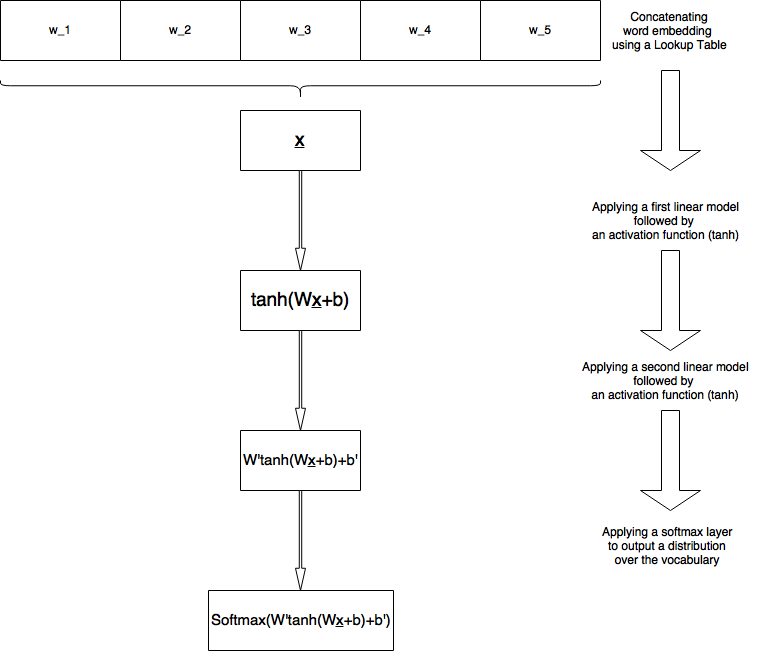
\includegraphics[width=0.4\textwidth]{reg.png}
    \caption{\underline{Neural Language Model (Bengio,2003)}}
\end{center}
\end{figure}

We then implemented a variant of the model using a skip-layer that concatenates the output of the tanh layer again with the original embeddings. The updated formula for the model is:

$$ nnlm_2(\boldsymbol{x}) = [\tanh(\boldsymbol{xW}+\boldsymbol{b}),\boldsymbol{x}]\boldsymbol{W'}+\boldsymbol{b'}$$

where this time:
\begin{itemize}
\item $\boldsymbol{W'}\in \Re^{(d_{hid}+ d_{in}\cdot d_{win})\times |\mathcal{V}|}$, and $\boldsymbol{b'}\in \Re^{|\mathcal{V}|}$
\end{itemize}

The updated diagram is as follows:
\begin{figure}[H]
\begin{center}
    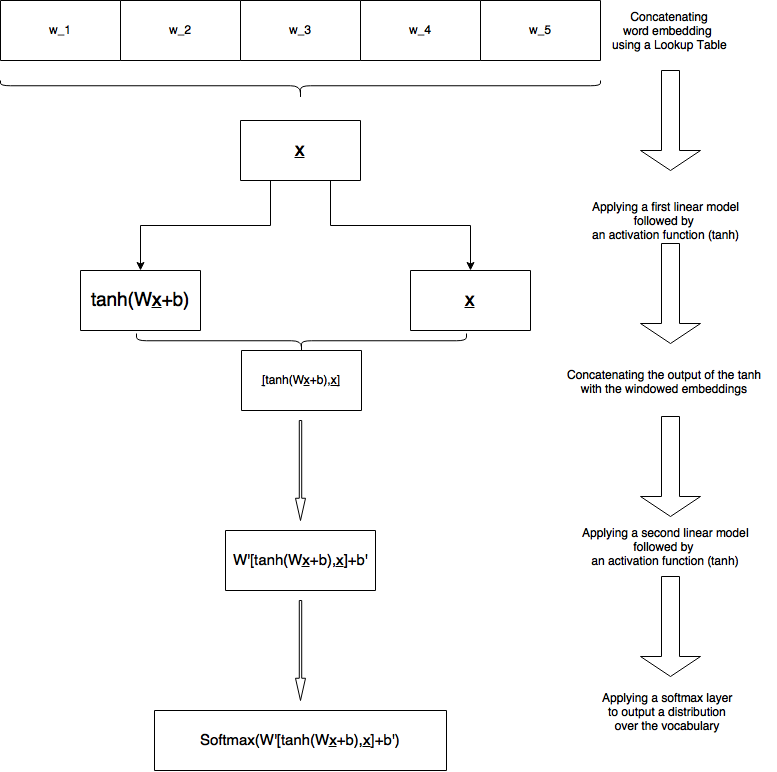
\includegraphics[width=0.5\textwidth]{skip.png}
    \caption{\underline{Skip-Layer Model}}
\end{center}
\end{figure}

We now show the pseudo code for training these NNLMs using batch stochastic gradient descent:
  \begin{algorithmic}[1]
    \Procedure{$NNLM_i$}{$win_{1},...,win_{n}$,MaxEpoch,BatchSize,LearningRate}
    \For{epoch = 1,MaxEpoch}
    \For{batch = 1, $|$train$|$/BatchSize}
    \For{win in batch}
    \State{Call $NNLM_i$:forward(win)}
    \State{Evalute the loss}
    \State{Evaluate derivatives of the loss}
    \State{Backprop through $NNLM_i$}
    \EndFor{}
    \State{Update Parameters with LearningRate}
    \EndFor{}
    
    \EndFor{}
    \EndProcedure{}
  \end{algorithmic}


\subsubsection{Noise Contrastive Estimation}

As mentioned earlier, training such model is extremely expensive in computation, especially on CPUs. The issue comes from the use of the softmax in the last layer of the model in order to obtain a distribution on a large vocabulary. In order to speed up the training time and reduce compution, we tried to implement NCE, which is a method used to fit unnomarlised method and therefore avoids using the last softmax layer.\\

\noindent The principle behind NCE is to sample for every context in the training data K wrong words that do not appear next in the windows using a noise distribution such a multinomial of the vocabulary simplex. We then apply a log-bilinear model. For a given context $\boldsymbol{x}$ and target $y$, the probability of $y$ being a correct word for this context is given by:
$$p(D = 1 | \boldsymbol{x,y}) =  \sigma(\log p(\boldsymbol{y}|D = 1,\boldsymbol{x})-\log Kp(\boldsymbol{y} | D = 0, \boldsymbol{x}))$$
where $$p(D = 1|\boldsymbol{x}, \boldsymbol{y}) = \sigma(log p(\boldsymbol{y}|D = 1, \boldsymbol{x}) - log(Kp(\boldsymbol{y}|D = 0, \boldsymbol{x})))
$$
If the $p(y|D = 1, x)$ term still forces some normalisation in the model, thanks to the contribution of Mnih and Teh (2012), we can estimate the normalisation constant as a parameter in the model and even set to equal to 1. We can therefore replace this term by the score outpute by the linear model $z_{\boldsymbol{x_i},w_i}$. The objective function that needs to be minimised becomes:

$$\mathcal{L}(\theta) = \sum\limits_{i} \log \sigma(z_{\boldsymbol{x_i},w_i}) - \log(K p_{ML}(w_i))) + \sum\limits_{k=1}^{K} \log(1-\sigma(z_{\boldsymbol{x_i},s_k}) - \log K p_{ML}(s_k)) $$

where $p_{ML}$ is the pdf of the noise distribution, and $s_k$ for $k \in \{1,...,K\}$ are samples from the noise distribution.
 
\section{Experiments}

We now present the results of our experiments. We will first talk about the preprocessing and then continue with a comparison of the different models.

\subsection{Data and Preprocessing}

To complete this homework, we were given 3 datasets, one for training, one for validation and one for testing. The train set consisted of sentences with a total of over eight hundred thousands words from a vocabulary of ten thousands words. The validation set consisted of 70391 words. The particularity of the issue at hand consisted in the fact that we had to only predict a probability distribution over 50 words and not on the entire vocabulary. This is why we were provided the same validation set in the same format as for the test set. We could therefore predict 3370 words on the validation set to help us predict the 3361 words of the test set.\\

\noindent Most of the preprocessing was about building the N-grams for the different sets. We included in the preprocess.py file different functions to evaluate the windows as well as counting the different occurences of each N-grams. For instance, looking at 6-grams gave:

\begin{itemize}
\item 772 670 unique 6-grams on the training set,
\item 887 522 6-grams in total,
\item 70 391 6-grams on the validation set,
\item 3 370 words to predict on the validation set,
\item and 3 361 words of the test set
\end{itemize}

\subsection{Evaluation}

To evaluate the models, we will use the perplexity measure. For a set of $m$ $N$-grams, $\boldsymbol{w}_1,...,\boldsymbol{w}_m$, it is defined to be:

$$ P(\boldsymbol{w}_1,...,\boldsymbol{w}_m) = \exp\left(-\frac{1}{m} \sum\limits_{i = 1}^{m} \log P(w_N^i|w_{N-1}^i,...,w_1^i)\right)$$

\noindent In other words, the perplexity translates how likely is the predicted word given the previous N-1 words. In this report, we will evaluated perplexity both on the entire vocabulary but also on the reduced 50 words to predict from. Values between these two "different" perplexities wil range from 3 to 1000.

\subsection{Count-based Models}

We evaluate the count-based models on the Kaggle development set with the perplexity.

\paragraph{Maximum Likelihood Estimation}

For this first model, the only hyperparameter is the number of N-grams in the feature. We applied this method on different N-gram models and provides the results. The computation time remains very low for each model; the only issue as we increase the size of the N-gram is the memory footprint.

\paragraph{Laplace Smoothing}

We studied the impact of the alpha parameter and the best value with regard to the perlexity on the Kaggle development set.

\begin{figure}[H]
  \centering
  \begin{minipage}[b]{0.45\textwidth}
    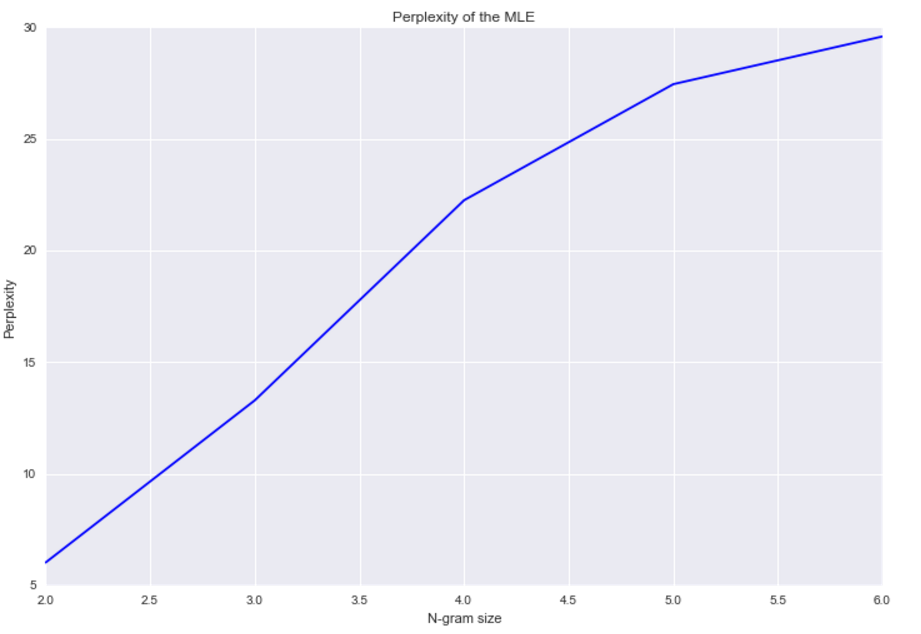
\includegraphics[width=\textwidth]{perp_mle}
  \end{minipage}
  \hfill
  \begin{minipage}[b]{0.45\textwidth}
    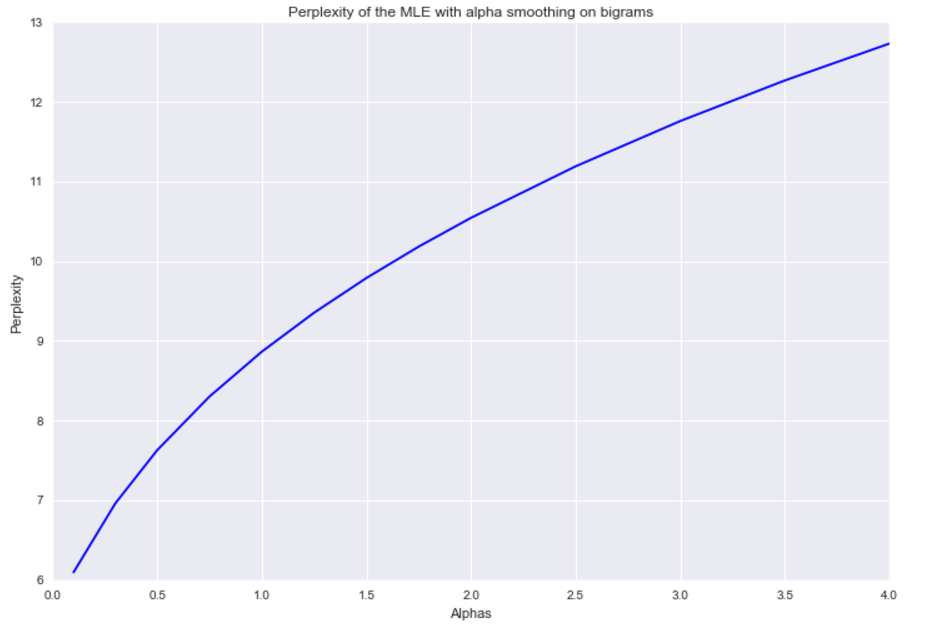
\includegraphics[width=\textwidth]{perp_alpha}
  \end{minipage}
\end{figure}


\paragraph{Witten-Bell Smoothing}

For the Witten-Bell Smoothing, we benchmarked both the alpha parameter and the context from which to start the interpolation.

First, we applied a different normalization when we were using our model for the Kaggle dataset. For each entry in this dataset, we build a language model on a really small subset of the training dictionary (50 out of 10 001 words). As a result, only a small fraction of all the N-grams can be considered and we decided to compute the factor $N1$ and $F_c$ only among the output vocabulary (50 words). This change lead to better results, we directly applied it on the modified Kneser-Ney.

\begin{figure}[H]
  \centering
  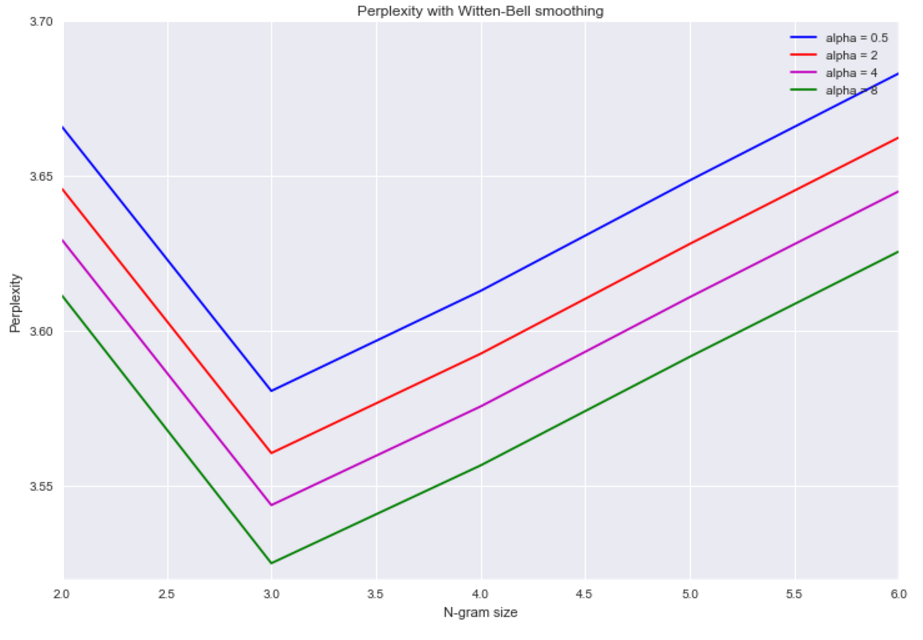
\includegraphics[width=0.45\textwidth]{perp_wb}
\end{figure}

This plots shows that the Witten-Bell smoothing does not manage to successfully balance the different orders of the models when they are too many. The best perplexity is always reached for the tri-grams. This may be cause by the fact that with large context (N>2), the probability may be disturbed by a lower order model very present even though the rest of the context is not (see the example of SAN FRANCISCO in the paper).

Moreover, we see that the perplexity gets smaller as $\alpha$ increases. This is because we may want a strong smoothing of the lower order model (here we use alpha only on the lower order model computed). The relative differences are bigger in the lower order models as the contexts are there more frequent (because smaller) so large smoothing may decrease their influence and favorise the long tail.

\paragraph{Modified Kneser-Ney}

This model introduces different hyperparameters. The absolute discounting D induces 2 kinds of hyperparameters: the number of values it takes and the values. We first applied those suggested in the paper but also decided to tune them manually as the paper provides better results in that case. We also observed this result.

We plot the results with a model with fixed parameters D as suggested in the paper. As with the Witten-Bell smoothing, we evaluated the models against different starting contexts. In that case, the best results were reached for the 3-grams.

\begin{figure}[H]
  \centering
  \begin{minipage}[b]{0.45\textwidth}
    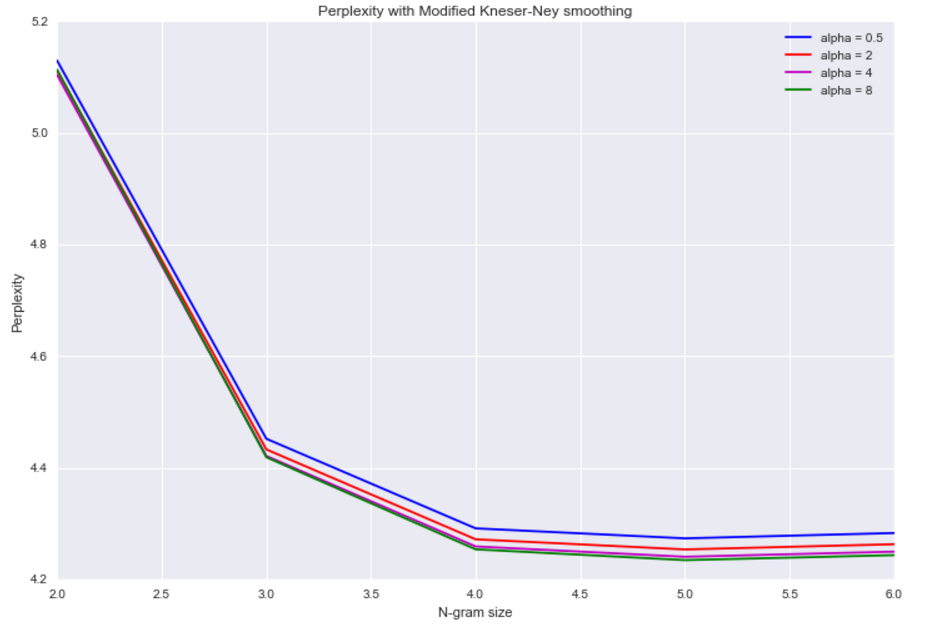
\includegraphics[width=\textwidth]{perp_mkn}
  \end{minipage}
  \hfill
  \begin{minipage}[b]{0.45\textwidth}
    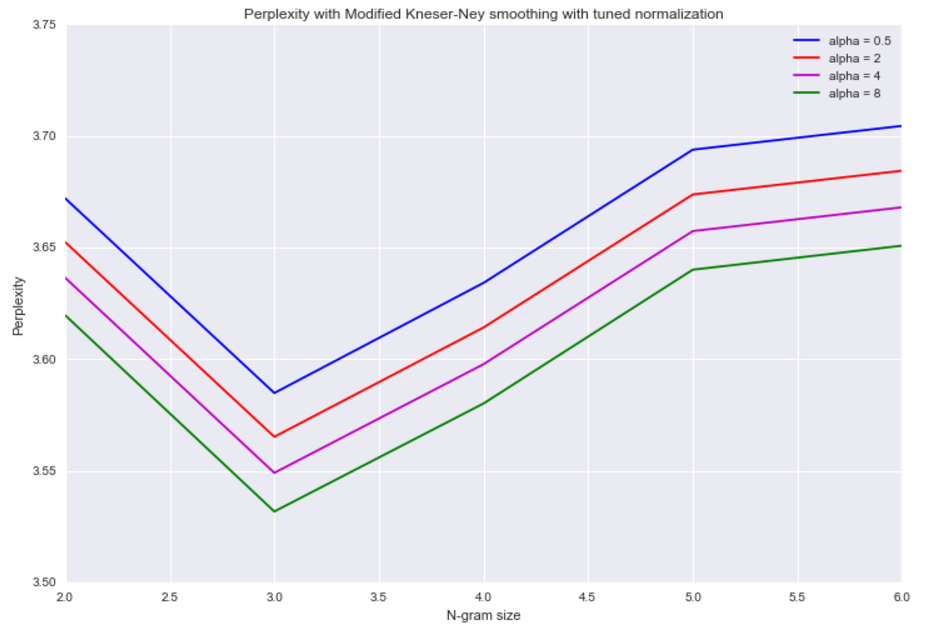
\includegraphics[width=\textwidth]{perp_mkn_norm}
  \end{minipage}
\end{figure}


The best perplexity was reached with a manually tuned D (on the Kaggle development set with the perplexity). The perplexity reached is $\mathbb{3.476}$.



\subsection{Neural Models}

The main issue we faced with Bengio's model was training time. Even we managed to have a working model with a smaller vocabulary, we struggled at first to get a code that ran fast enough to experiment extensively with different paremetrisations. Our original code ran one epoch in about one hour for the paremetrisation. While trying to code the NCE approximation, we nevertheless managed to cut the training time to about 14-15 minutes.\\

We started to train the more simple neural network i.e. the one without the skip-layer, with the parametrisation suggested by Bengio:

\begin{itemize}
\item Window size: $d_{win} = 5$
\item Dimension of the embeddings: $d_{in} = 30$
\item Hidden dimension: $d_{hid} = 100$
\end{itemize}

We summarize the results in the graphs below:

\begin{figure}[H]
  \centering
  \begin{minipage}[b]{0.45\textwidth}
    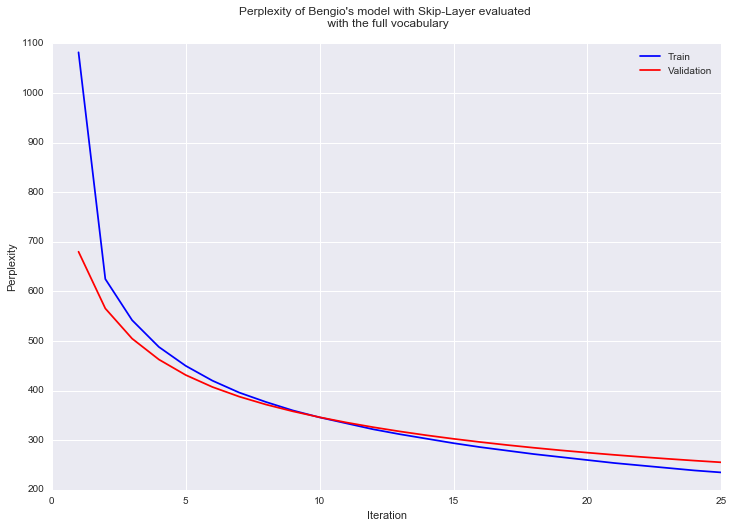
\includegraphics[width=\textwidth]{noskip_tr}
  \end{minipage}
  \hfill
  \begin{minipage}[b]{0.45\textwidth}
    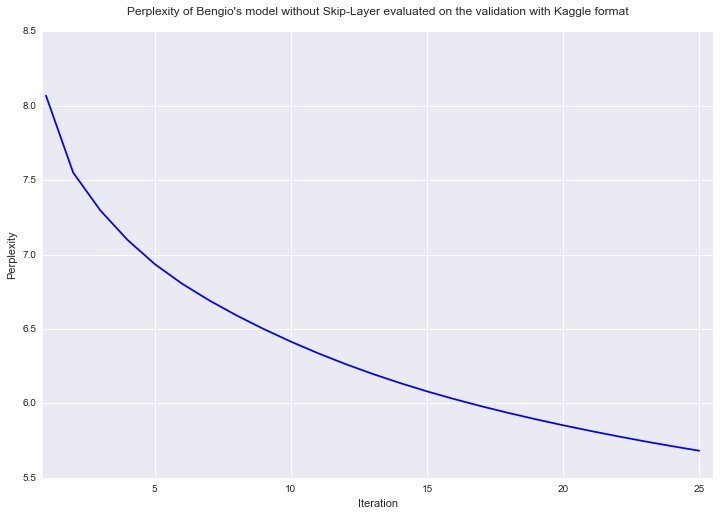
\includegraphics[width=\textwidth]{noskip_val}
  \end{minipage}
\end{figure}

Before making a submission on kaggle, we decided to compare the encouraging results with the Skip-Layer model. We ran the experiment 5 epochs at a time to give us control on the learning rate. We thought that after the 15 epochs, the model was close to convergence, and decided to decrease the learning rate from 0.01 to 0.001. We obtain the following results:
\begin{figure}[H]
  \centering
  \begin{minipage}[b]{0.45\textwidth}
    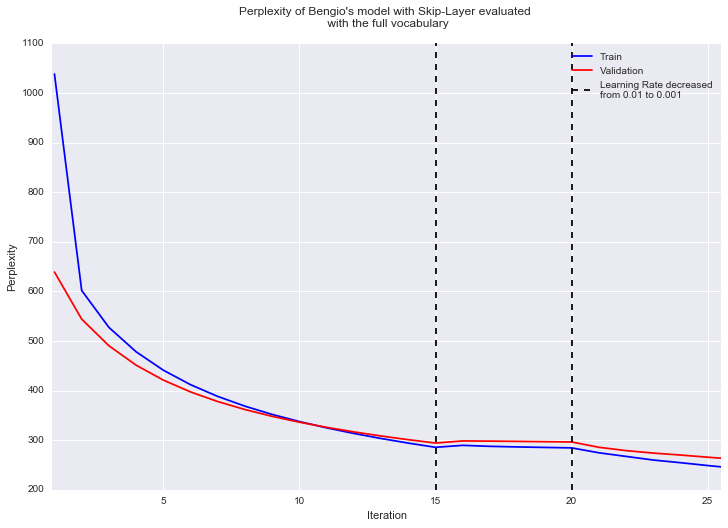
\includegraphics[width=\textwidth]{skip_tr}
  \end{minipage}
  \hfill
  \begin{minipage}[b]{0.45\textwidth}
    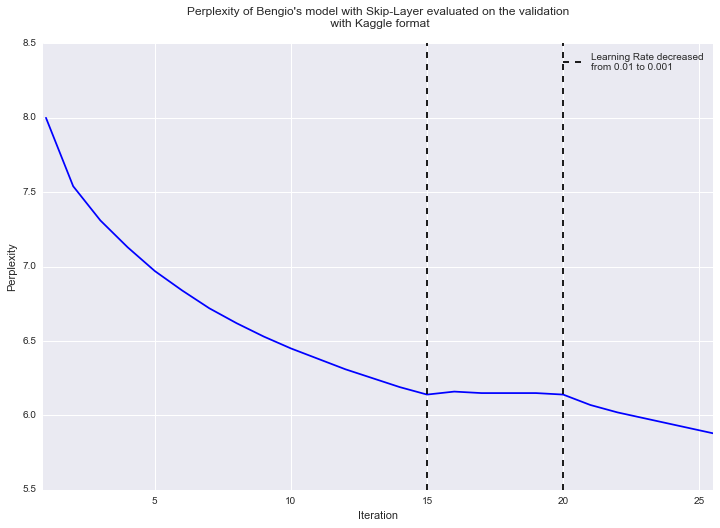
\includegraphics[width=\textwidth]{skip_val}
  \end{minipage}
\end{figure}

\noindent As one can see, changing the learning rate negatively impacted the results. It plateaued but perplexity started decreasing again as soon as we re-up the learning rate. It also unclear how much improvement the skip-layer model brings compared to the original Bengio model, and this even without the change in learning rate. Based on these observation, we decided to submit to Kaggle the results of the simple model. We obtained:

$$Perp^{test}_{nnlm} = 5.47$$

\noindent Nevertheless, a final observation on the training of these NNLMs is that the models haven't seem to converge fully after 25 epochs. Running the algorithm for 5-10 extra epochs would most probably yielded better results and helped us reach the level of the count-base models.

\subsection{NCE}

We unfortunately did not succeed to implement a valid version of the Noise Contrastive Estimation. We did not managed to have a speed improvement and even worse observed that the perplexity on the validation was increasing instead of decreasing.

\subsection{Mixtures of models}
In order to increase our score, we decided to combine the differente approaches by averaging the results over the distributions outputted by various models.

We managed to reach our best perplexity with a weigthed mean of the Witten-Bell smoothing, the modified Kneser-Kney with tuned parameters and local normalization and the Neural Network.

Formallu, the output is built as follows:

\[
p(w|c) = \frac{2p_{WB}(w|c) + p_{mKN}(w|c) + p_{NN}(w|c)}{5}
\]

We reached on the Kaggle development set: $ \mathbb{perp_{Kaggle} = 3.36}$

We provide here a summary of our models on the Kaggle development set:


\begin{table}[]
\centering
\caption{My caption}
\label{my-label}
\begin{tabular}{|l|l|}
\hline
Model                          & Perplexity (dev Kaggle) \\ \hline
MLE with Laplace smoothing     & 6.01                    \\ \hline
Witten Bell (trigram)          & 3.52                    \\ \hline
Modified Kneser Kney           & 3.47                    \\ \hline
Neural Network                 & 5.68                    \\ \hline
Neural Network with skip Layer & 5.66                    \\ \hline
Ensemble (WB + mKN + NNsl)     & \textbf{3.36}                    \\ \hline
\end{tabular}
\end{table}


\section{Conclusion}

End the write-up with a very short recap of the main experiments and the main results. Describe any challenges you may have faced, and what could have been improved in the model.

\section{References}
\begin{itemize}
\item Bengio, Y., Ducharme, R., Vincent, P., and Janvin, C. (2003). A neural probabilistic language model. \emph{Journal of Machine Learning Research}, 3:1137–1155.

\item Mnih, A. and Kavukcuoglu, K. (2013). Learning word embeddings efficiently with noise- contrastive estimation. \emph{In Advances in Neural Information Processing Systems}, pages 2265–2273.

\item Chen, S. and Goodman, J. (1998). An Empirical Study of Smoothing Techniques for Language. \emph{Technical Report TR-10-98}, Computer Science Group, Harvard University.
\end{itemize}

\newpage

\begin{appendices}
\lstinputlisting{../preprocess.py}
\lstinputlisting{../count_models.lua}
\lstinputlisting{../bengio_nn.lua}
\end{appendices}

\end{document}

